\documentclass{article}
% Formatting: the ICLR 2026 style files (iclr2026_conference.sty and .bst), used for their look
% only. This preprint was not submitted to ICLR; the conference header is cleared below.
\usepackage{iclr2026_conference,times}
\iclrfinalcopy

\usepackage[T1]{fontenc}
\usepackage[utf8]{inputenc}
\usepackage{inconsolata}
\usepackage{microtype}
\usepackage{amsmath,amssymb}
\usepackage{booktabs}
\usepackage{tabularx}
\usepackage{graphicx}
\usepackage{xcolor}
\usepackage{enumitem}
\usepackage{hyperref}
\usepackage{url}

\setlist{itemsep=2pt,topsep=4pt}
\setlength{\emergencystretch}{2em}
\newcommand{\cond}[1]{#1}
\newcommand{\ci}[2]{\,{\small(#1--#2)}}

\title{Calibrated but Timid: Fine-Tuned Decision Models as the Learn Stage of LLM-Generated Rule Pipelines for Founder Screening}
\author{Siddarth Oruganti \\
Imperial College London \\
\texttt{siddarth.oruganti26@imperial.ac.uk}}

\begin{document}
\maketitle
\lhead{}  % a preprint: no conference header, only the rule

\begin{abstract}
Think--Reason--Learn (TRL) pipelines predict whether a startup founder will succeed in three
steps: a large language model writes yes/no questions about founders (\emph{think}), a model
answers them for each founder (\emph{reason}), and a classical model combines the answers into
a prediction (\emph{learn}). We ask which learn stage gives the most accurate and best-calibrated
predictions when the think and reason steps are held fixed. We add a TRL-native
\emph{decision combiner}, which hands the final step to a decision model, and compare eight
conditions on 3,000 anonymised founder profiles (50 grounded in real founders, 2,950 synthetic):
TRL's elastic net and vote, XGBoost, and the open 0.6B-parameter decision model Kev, zero-shot
and fine-tuned, reading either TRL's answers or the raw profile. All conditions share the same 93
LLM-written questions and the same answer matrix. Thresholds are tuned on validation, the 600
test founders are scored once, and every comparison is a paired bootstrap. No learn stage beats
TRL's default elastic net (F0.5 0.319, 95\% CI 0.221--0.417): every paired F0.5 difference
includes zero. Fine-tuning cuts Kev's expected calibration error from 0.262 to 0.012, the lowest
of any condition, but compresses its probabilities (none above 0.39), which costs recall at a
precision-favouring threshold. A noise-free oracle from the synthetic generator reaches PR-AUC
0.328 against the elastic net's 0.304, so there is little headroom on this data. Kev reading
the raw profile matches Kev reading TRL's answers. Finally, a multi-output production model's
predictions shift by up to 0.18 when its choice options are sent without the descriptions it was
trained with, a pitfall we fix in TRL. Code, data, models and every result are released.
\end{abstract}

\section{Introduction}

Angel investors screen most founders alone, with little time and no analysts. An automated
first pass could help, but only if its numbers can be trusted: an agent that advances or passes
founders on the investor's behalf needs probabilities that mean what they say, so that a
threshold can be chosen for a target precision. Accuracy alone is not enough; \emph{calibration}
is what makes autonomous action safe~\citep{guo2017calibration}.

Think--Reason--Learn (TRL), Vela Research's open-source framework~\citep{trl}, offers
interpretable, scikit-learn-compatible classifiers built from LLM-generated rules. Its Random
Rule Forest (RRF)~\citep{trlresearch} asks an LLM to write yes/no questions that separate
successful from unsuccessful founders, answers each question for every founder, and combines
the answers with an elastic-net logistic regression~\citep{zou2005elasticnet} or a vote. The
questions make each prediction explainable; the combiner is deliberately simple.

Decision models such as TypeSafe's Jev~\citep{jev} and its open reconstruction Kev~\citep{kev}
return calibrated probabilities over options defined in the request, with no text output. They
are already used as TRL's \emph{answerer}. This raises a natural question: should a decision
model also make the final call? It could combine answers non-linearly, be fine-tuned on exactly
the text it reads, and be calibrated by temperature scaling.

\paragraph{Research question.} With the think and reason steps held fixed, which learn stage
gives the most accurate (F0.5) and best-calibrated (ECE, Brier) predictions of founder success?

\paragraph{Contributions.}
\begin{enumerate}
\item A TRL-native \emph{decision combiner} (\texttt{RRF(combiner="decision")}) that serialises
  RRF's answers as text and asks a decision model for P(success), with TRL's own threshold
  tuning, tests and cost estimation (Section~\ref{sec:combiner}).
\item A controlled comparison of eight conditions on identical questions and answers: TRL's
  elastic net (all questions, and the same 40 Kev reads), the RRF vote, XGBoost, and Kev-0.6B
  zero-shot and fine-tuned, reading TRL's answers or the raw profile, with paired bootstrap
  confidence intervals (Sections~\ref{sec:setup}--\ref{sec:results}).
\item Evidence that fine-tuning makes a small decision model the best-calibrated learn stage
  without improving discrimination, and that its probabilities are compressed (``timid''), which
  matters for threshold-based policies (Section~\ref{sec:results}).
\item A ceiling analysis using the synthetic generator's noise-free score, showing how close
  every learn stage already is to the attainable ranking (Section~\ref{sec:ceiling}).
\item A practical finding for decision-model pipelines: the options' descriptions in the request
  move a fine-tuned model's distributions by up to 0.18; we fix TRL to send them
  (Section~\ref{sec:production}).
\end{enumerate}

\section{Background and related work}

\paragraph{TRL and RRF.} TRL~\citep{trl} implements several LLM-rule methods behind one provider
layer and a scikit-learn interface. RRF has an LLM generate many candidate yes/no questions from
training examples (by default 10 prompts of 10 questions, each prompt seeing 30 balanced
examples), scores each question by F-beta on train, and fits a combiner on the answer matrix.
The library default is an elastic-net logistic regression; the method's paper and its VCBench
entry~\citep{vcbench} use a vote (predict success when at least $T$ of the top $N$ questions are
answered yes). The approach resembles concept-bottleneck models~\citep{koh2020concept}, with the
concepts written by an LLM and answered by a model rather than annotated.

\paragraph{Decision models.} Jev (TypeSafe's ``System One'') returns a probability for each
option of each question in a request, given a free-text \emph{state}~\citep{jev}. Kev~\citep{kev}
reconstructs its design openly: a Qwen3 base model~\citep{qwen3} with a rank-16
LoRA~\citep{hu2022lora} and a pointer head that scores each option's end-of-option hidden state
against the hidden state of a \texttt{<decide>} token, followed by a softmax and a fitted
temperature. The released \texttt{kev-0.6b} checkpoint is uncalibrated (temperature 1.0) and
serves TypeSafe's \texttt{/v1/systemone} API.

\paragraph{Calibration.} We measure calibration with the Brier score~\citep{brier1950} and the
expected calibration error (ECE) over 10 equal-width bins~\citep{naeini2015ece}, and calibrate Kev
by temperature scaling on validation~\citep{guo2017calibration}. Because successes are a minority
(20\%), we report PR-AUC as the threshold-free ranking measure~\citep{saito2015prc}.

\section{Data}
\label{sec:data}

\paragraph{Profiles.} Each record is an anonymised founder profile in a fixed template, true as of
the company's founding date: the startup's industry and number of co-founders; the founder's
background (technical, business, mixed or domain specialist), years of experience and depth of
industry experience; one to three education entries (degree, field, QS-rank band); one to six
jobs (role, generic employer description, size band, industry, duration band); and prior
startups and exits with value bands. No names, dates, places or post-founding facts appear. Each
record is labelled with the outcome band as of 2025 (shut down, under \$50M, \$50M--\$500M,
\$500M--\$1B, over \$1B) and years to that outcome (under 5, 5--8, over 8).

\paragraph{Construction.} Fifty profiles are grounded in real founders and companies founded
2010--2019, with outcomes checked against public records (38 of 50 re-verified by web search; the
rest from the public record). The other 2,950 are generated by a seeded program modelled on them
(roughly 80 industries, career pools by background, consistency rules between experience, jobs,
degrees and exits). A synthetic founder's outcome comes from a \emph{background score}, a mostly
additive function of the profile (industry, industry experience, prior exits, team size,
education rank, big-company experience, background) with five small interaction terms, plus
Gaussian noise ($\sigma = 0.62$). Within each block of 50, the noisy scores are ranked and cut
into exact band counts (25/8/7/5/5, alternating 7/8), and years are drawn per band. About 16\% of
rows mark one or two fields as unknown. The noise level was chosen so that a logistic model on
the profile fields reaches AUC 0.69 and the best single field 0.59, far from the ``too easy''
line we set in advance (0.8 F0.5).

\paragraph{Label and splits.} The research label is \emph{success}: an outcome of \$500M or more
(20\%). The 3,000 rows are split 2,000 / 400 / 600 (train / validation / test), stratified on
outcome band (seed 42), with exact and near-duplicate profiles ($\geq$80\% shared five-word
shingles) kept in one split. Test has 120 successes and validation 80.

\section{Methods}
\label{sec:setup}

\subsection{The fixed think and reason steps}

All conditions use TRL 0.3.0 (upstream commit \texttt{3437d64}) from our fork, and every model
call goes through TRL's \texttt{RRF}, \texttt{LLM} and \texttt{LLMSession} with TRL's disk cache.
RRF uses library defaults except $\beta = 0.5$ (F0.5, the VCBench metric) and
\texttt{random\_state=42}. The task given to TRL is ``Predict whether this startup founder's
company will succeed (exit, IPO or funding over \$500M).''

\paragraph{Think.} Claude Opus 5.5 wrote the questions from the 2,000 training founders: 93
distinct yes/no questions (for example, ``Did the founder spend 5+ years at a single employer in
the same industry as the current startup?''). The question generation cost \$0.49.

\paragraph{Reason.} The released Kev-0.6B answers every question for every founder, served by
\texttt{kev.serve} in fp32 on a free Kaggle T4 (about 104 answers per second through TRL) and
reached as \texttt{LLM("kev-0.6b", base\_url=".../v1/systemone", kind="decision")}. Kev replaces
Jev, TRL's default answerer, because Jev has no free tier. The answer matrices (P(yes) per founder
and question) are computed once and cached; none is missing.

\paragraph{The best 40.} Decision-model conditions read the 40 questions with the best train F0.5
(TRL's \texttt{max\_rules=40}). This keeps each serialised state near 900 tokens rather than
about 3,000, which makes fine-tuning on a T4 feasible. The elastic net on the same 40
(\cond{C1a-40}) isolates the learn stage from this cap.

\subsection{The decision combiner}
\label{sec:combiner}

We add \texttt{RRF(combiner="decision", combiner\_model=..., combiner\_question=...)} to TRL. For
each founder, RRF's answers are written as text, one line per rule in rule order, the question
followed by \texttt{yes} (P(yes) $\geq 0.5$), \texttt{no}, or \texttt{unknown} when unanswered
(TRL's new \texttt{answers\_text}, so training data and prediction use the same function). The
decision model is asked one yes/no question about that text (``Will this founder's company succeed
(exit, IPO or funding over \$500M)?''), and its probability is the score. \texttt{fit} tunes the
threshold with TRL's \texttt{best\_threshold}, as the other combiners do. The combiner stores its
constructor arguments unchanged, passes TRL's \texttt{check\_classifier} and contract tests
offline, and counts the decision model's calls in \texttt{estimate\_cost}.

\subsection{Conditions}

\begin{table}[t]
\centering\small
\caption{The eight conditions. All read the same founders; the answer-based ones read the same
questions and answers.}
\label{tab:conditions}
\begin{tabularx}{\textwidth}{@{}l X l l@{}}
\toprule
ID & Learn stage & Reads & Trained on \\
\midrule
\cond{C1a} & RRF elastic net (TRL default) & all questions' answers (63 kept) & train \\
\cond{C1a-40} & RRF elastic net, \texttt{max\_rules=40} & the best 40 answers & train \\
\cond{C1b} & RRF vote (the paper's method) & its selected questions (21) & train \\
\cond{CTRL} & XGBoost & the best 40 answers & train (tuned on val) \\
\cond{C2} & base Kev-0.6B, decision combiner & the best 40, as text & nothing \\
\cond{C3} & fine-tuned Kev-0.6B, decision combiner & the best 40, as text & train \\
\cond{C4} & fine-tuned Kev-0.6B, no questions & the profile as TRL renders it & train \\
\cond{EXTRA} & base Kev-0.6B, no questions & the profile as TRL renders it & nothing \\
\bottomrule
\end{tabularx}
\end{table}

Table~\ref{tab:conditions} lists the conditions. \cond{CTRL} separates ``Kev helps'' from ``any
non-linear learner helps'': XGBoost~\citep{chen2016xgboost} over a grid of depth $\{2,3,4\}$
$\times$ learning rate $\{0.03, 0.1\}$ $\times$ minimum child weight $\{1,5\}$, up to 2,000 trees
with early stopping on validation log-loss (chosen: depth 2, rate 0.1, child weight 5).
\cond{C4} and \cond{EXTRA} read exactly the text TRL sends its answerer, so they differ from the
TRL conditions only by skipping the think and reason steps.

\subsection{Fine-tuning and calibration}

\cond{C3} and \cond{C4} are fine-tuned with Kev's own trainer from the released checkpoint, with
its architecture copied from the checkpoint metadata (LoRA rank 16 on all targets, head dimension
256): learning rate $2\times10^{-5}$, batch 8, fp32 (the T4 has no bf16), seed 42, and a maximum
state length of 4,096 tokens. Kev's default of 384 would silently drop every \cond{C3} record.
Each model trains one epoch from the release and a second from the first; the checkpoint with the
lowest validation log-loss among the release, epoch 1 and epoch 2 is kept, and one temperature is
fitted on validation by minimum log-loss.

\subsection{Evaluation protocol}

Every condition uses one threshold rule: the F0.5-best threshold on validation (TRL's
\texttt{best\_threshold}), applied unchanged to test. For \cond{C1a}, \cond{C1a-40} and
\cond{C1b} we also report TRL's as-shipped decision (threshold tuned out of fold on train).
On test we report F0.5, precision, recall, Brier, ECE (10 equal-width bins, weighted) and PR-AUC,
with 95\% percentile intervals from 1,000 stratified bootstrap resamples (positives and negatives
resampled separately) with the threshold held fixed~\citep{efron1993bootstrap}. Comparisons
between conditions use a \emph{paired} stratified bootstrap of the difference on the same
resampled founders. The pairs were fixed from the research question before any test score was
computed. The validation-only results, and the choice of the production model's input
(Section~\ref{sec:production}), were committed before test was read once.

\section{Results}
\label{sec:results}

\begin{table}[t]
\centering\small
\caption{Test results (600 founders, 120 successes; a random pick succeeds 20\% of the time).
Thresholds tuned on validation for F0.5. 95\% stratified bootstrap CIs in brackets. Best value
per column in bold.}
\label{tab:main}
\resizebox{\textwidth}{!}{%
\begin{tabular}{@{}l c c c c c c@{}}
\toprule
Condition & F0.5 & Precision & Recall & Brier $\downarrow$ & ECE $\downarrow$ & PR-AUC \\
\midrule
\cond{C1a} elastic net & \textbf{0.319}\ci{0.221}{0.417} & \textbf{0.383} & 0.192 & \textbf{0.153} & 0.045\ci{0.027}{0.076} & \textbf{0.319}\ci{0.270}{0.395} \\
\cond{C1a-40} elastic net, 40 & 0.306\ci{0.236}{0.378} & 0.312 & 0.283 & 0.156 & 0.035\ci{0.024}{0.072} & 0.286\ci{0.245}{0.353} \\
\cond{C1b} vote & 0.305\ci{0.249}{0.354} & 0.286 & 0.417 & 0.249 & 0.251\ci{0.232}{0.273} & 0.264\ci{0.228}{0.316} \\
\cond{CTRL} XGBoost & 0.305\ci{0.205}{0.399} & 0.375 & 0.175 & 0.154 & 0.040\ci{0.024}{0.075} & 0.317\ci{0.269}{0.393} \\
\cond{C2} base Kev, answers & 0.277\ci{0.242}{0.312} & 0.244 & \textbf{0.608} & 0.230 & 0.262\ci{0.251}{0.271} & 0.268\ci{0.230}{0.332} \\
\cond{EXTRA} base Kev, profile & \textbf{0.319}\ci{0.246}{0.394} & 0.322 & 0.308 & 0.408 & 0.465\ci{0.446}{0.483} & 0.259\ci{0.225}{0.318} \\
\cond{C3} tuned Kev, answers & 0.227\ci{0.121}{0.332} & 0.333 & 0.100 & 0.156 & \textbf{0.012}\ci{0.008}{0.045} & 0.285\ci{0.242}{0.352} \\
\cond{C4} tuned Kev, profile & 0.282\ci{0.191}{0.368} & 0.333 & 0.175 & 0.155 & 0.021\ci{0.014}{0.051} & 0.285\ci{0.241}{0.349} \\
\bottomrule
\end{tabular}}
\end{table}

Table~\ref{tab:main} gives the test results and Figure~\ref{fig:paired} the planned paired
comparisons.

\paragraph{No learn stage beats the elastic net.} TRL's default (\cond{C1a}) scores 0.319 F0.5:
about 4 in 10 of the founders it flags succeed, against 2 in 10 at random. Every paired F0.5
difference against it includes zero: XGBoost $-0.014$ ($-0.096$ to $+0.071$), base Kev $-0.042$
($-0.127$ to $+0.046$), fine-tuned Kev on the answers $-0.092$ ($-0.206$ to $+0.012$) and on the
profile $-0.037$ ($-0.133$ to $+0.060$). Threshold-free ranking agrees: \cond{CTRL} matches
\cond{C1a} in PR-AUC ($-0.002$), and fine-tuned Kev trails it by $-0.034$ ($-0.085$ to $+0.017$).
Against the elastic net on the same 40 questions, fine-tuned Kev is level in PR-AUC ($-0.001$).
Neither trees nor a language model extract more from the answers than a weighted sum does.
\cond{C1a} with TRL's own out-of-fold threshold scores 0.312 (0.218--0.404), so tuning on
validation changes little.

\begin{figure}[t]
\centering
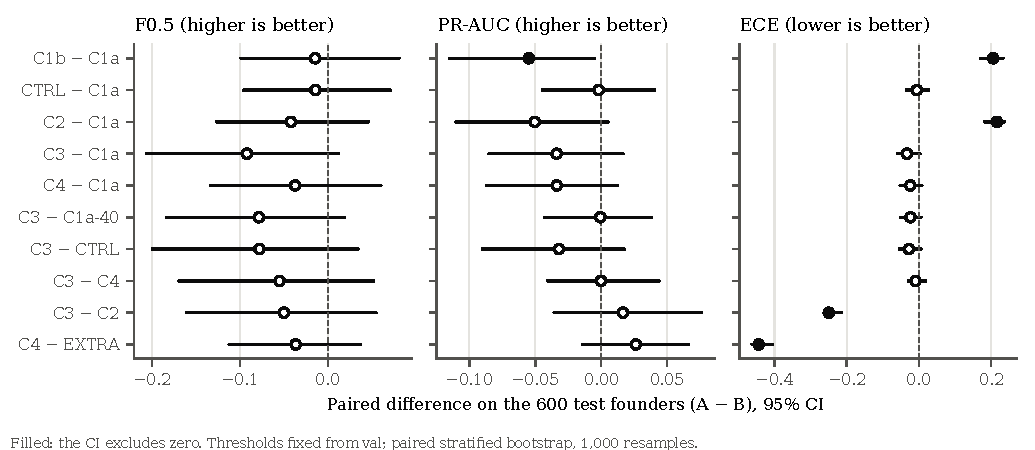
\includegraphics[width=\textwidth]{figures/paired_differences.pdf}
\caption{Planned paired comparisons on test (A $-$ B, 95\% paired bootstrap CI). Filled markers:
the interval excludes zero. No condition differs from \cond{C1a} in F0.5; fine-tuning (\cond{C3}
$-$ \cond{C2}, \cond{C4} $-$ \cond{EXTRA}) sharply reduces calibration error.}
\label{fig:paired}
\end{figure}

\paragraph{Fine-tuning makes Kev the best-calibrated learn stage.} The released Kev is badly
calibrated as a learn stage: ECE 0.262 reading TRL's answers (\cond{C2}) and 0.465 reading the
profile (\cond{EXTRA}), where it gives over 0.9 to founders who succeed about 3 times in 10.
Fine-tuning reduces ECE to 0.012 (\cond{C3}; paired difference $-0.249$, CI $-0.258$ to $-0.215$)
and 0.021 (\cond{C4}; $-0.444$, CI $-0.462$ to $-0.407$), with Brier improving by 0.074 and 0.253.
\cond{C3}'s ECE is the lowest of any condition, though its difference from \cond{C1a}'s 0.045 does
not exclude zero ($-0.033$, CI $-0.059$ to $+0.003$). Figure~\ref{fig:reliability} shows the
reliability curves.

\begin{figure}[t]
\centering
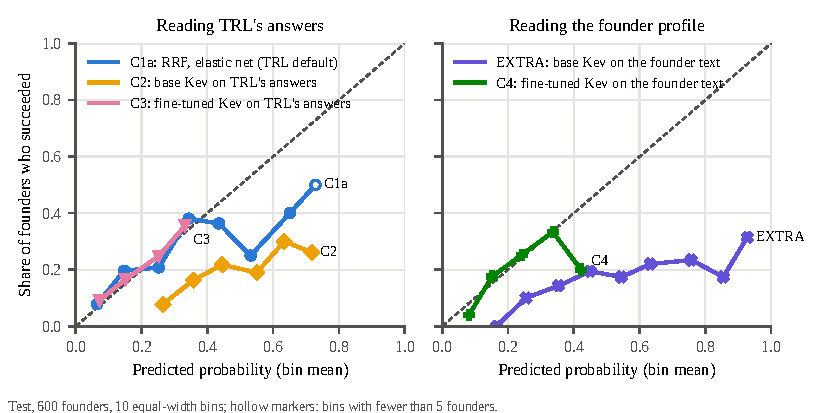
\includegraphics[width=\textwidth]{figures/reliability.pdf}
\caption{Reliability on test. Left: learn stages reading TRL's answers. The released Kev
(\cond{C2}) is over-confident; after fine-tuning (\cond{C3}) it lies on the diagonal, but only
between 0.05 and 0.40. Right: Kev reading the profile, before (\cond{EXTRA}) and after
(\cond{C4}) fine-tuning.}
\label{fig:reliability}
\end{figure}

\paragraph{But its probabilities are timid.} Fine-tuned Kev compresses its scores towards the base
rate: on test, \cond{C3} never exceeds 0.385 and \cond{C4} never exceeds 0.458, while the elastic
net reaches 0.745 (Figure~\ref{fig:scores}). Kev has learned the base rate and a modest shift
around it. Few founders clear a precision-favouring threshold, so \cond{C3} flags 36 of 600 and
finds 10\% of the successes (\cond{C1a}: 60 flagged, 19\%). This, rather than worse ranking,
drives its lower F0.5. The threshold, tuned on validation's 80 successes, is fragile: \cond{C3}'s
flagged founders succeed at 0.59 on validation but 0.33 on test.

\begin{figure}[t]
\centering
\begin{minipage}[t]{0.49\textwidth}
\centering
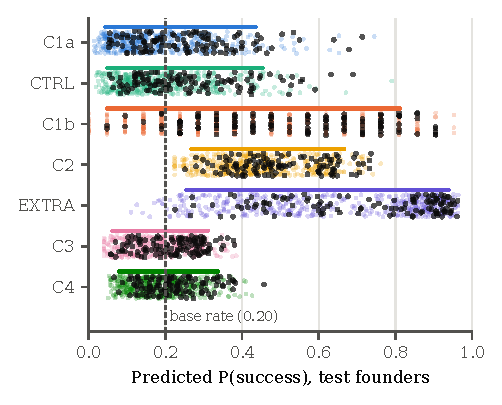
\includegraphics[width=\linewidth]{figures/score_ranges.pdf}
\caption{Predicted P(success) on test. Coloured dots: founders who did not succeed; black dots:
founders who did; bar: 5th--95th percentile. Fine-tuned Kev (\cond{C3}, \cond{C4}) stays close
to the 0.20 base rate; released Kev (\cond{C2}, \cond{EXTRA}) and the vote (\cond{C1b}) spread
far above it.}
\label{fig:scores}
\end{minipage}\hfill
\begin{minipage}[t]{0.49\textwidth}
\centering
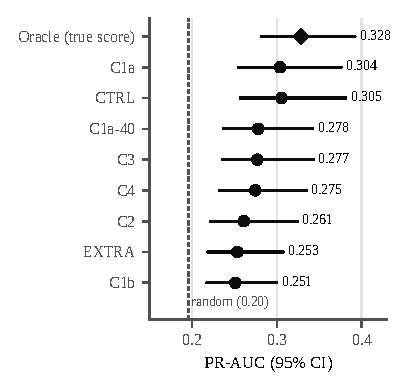
\includegraphics[width=\linewidth]{figures/ceiling.pdf}
\caption{PR-AUC on the 587 synthetic test founders (115 successes), with 95\% bootstrap CIs. The
oracle ranks founders by the generator's noise-free background score; the elastic net reaches
93\% of it.}
\label{fig:ceiling}
\end{minipage}
\end{figure}

\paragraph{TRL's questions explain more than they predict here.} Kev fine-tuned on the raw profile
(\cond{C4}) matched Kev fine-tuned on TRL's answers (\cond{C3}): identical PR-AUC (0.285), Brier
(0.155 against 0.156) and a paired F0.5 difference of $-0.055$ ($-0.169$ to $+0.052$). On
validation the two were tied (0.426 against 0.428). The profiles are short (about 170 tokens) and
templated, which favours reading them directly; the questions' value on this data is that each
prediction can be traced to named, human-readable factors.

\paragraph{The vote is not a probability.} The RRF paper's vote (\cond{C1b}) ranks almost as well
as the elastic net in F0.5 ($-0.015$) but is far worse calibrated (ECE $+0.206$, CI $+0.170$ to
$+0.233$) and ranks worse (PR-AUC $-0.055$, CI $-0.115$ to $-0.005$): when it scores 0.9, about 4
in 10 succeed.

\paragraph{The cost of 40 questions.} Restricting the elastic net to the 40 questions Kev reads
costs a little ranking (PR-AUC $-0.033$, CI $-0.071$ to $-0.000$) but no detectable F0.5
($-0.014$).

\paragraph{Validation to test.} Every condition scores lower on test than on validation
(\cond{C1a}: 0.446 to 0.319), including \cond{C1a} with TRL's out-of-fold threshold (0.432 to
0.312), which is not tuned on validation at all. The drop is therefore most likely a property of
the splits (80 against 120 successes), not over-tuning. Appendix Table~\ref{tab:val} gives the
validation results.

\section{How much headroom is there?}
\label{sec:ceiling}

Because the synthetic outcomes come from a known rule, the generator's noise-free background
score is close to the best predictor obtainable from the profile. We regenerate the dataset (byte
for byte, seed 42) with each row's score and rank the 587 synthetic test founders by it
(Figure~\ref{fig:ceiling}). The oracle reaches PR-AUC 0.328 (0.282--0.392) and F0.5 0.361 with a
validation-tuned threshold. On the same founders the elastic net reaches 0.304 and XGBoost 0.305,
93\% of the oracle, and fine-tuned Kev 0.277. The oracle is not a strict bound (ranking within
blocks of 50 makes the label depend on neighbours, and test is finite), but the picture is clear:
the noise we injected, chosen to keep the task realistic, leaves little for any learn stage to
gain, and the generating rule is largely additive, which suits a linear combiner. A learn stage
that could find interactions would need data where interactions carry more of the signal.

\section{A production model, and a request-format pitfall}
\label{sec:production}

The product built on this research (a deal-screening agent for angel investors) needs more than
P(success): the investor chooses a target outcome and a timeline. We therefore trained one more
Kev with \cond{C3}'s input, chosen on validation before test was read (\cond{C3} and \cond{C4} were
tied; \cond{C3}'s input lets each verdict cite the questions that drove it). Instead of one yes/no
question it answers two \emph{choice} questions, \texttt{outcome} (five bands) and \texttt{years}
(three bands), each option carrying a one-line description (for example ``shut down: the company
closed''). Same recipe, two epochs of 87 minutes; validation log-loss (mean over the two
questions) fell from 2.010 (released Kev) to 1.163, and per-question temperatures of 1.149
(outcome) and 0.871 (years) brought ECE from 0.027 to 0.021.

\paragraph{It costs nothing measurable.} Summing the two top bands gives P(\$500M or more). On
validation it ranks founders about as well as \cond{C3}'s single yes/no answer (PR-AUC 0.357
against 0.403; paired difference $-0.047$, CI $-0.114$ to $+0.026$; ECE 0.040 against 0.024,
difference CI $-0.028$ to $+0.033$), the two scores correlate at 0.94, and the mean predicted share
of every band is within 2 points of the actual share.

\paragraph{Ask the model exactly as it was trained.} Our first scoring pass went through TRL, whose
System One adapter sent a choice question's options with empty descriptions. Asked that way, the
same checkpoint put 35\% on ``shut down'' on average instead of 52\% (actual 50\%), individual
distributions moved by up to 0.18, and log-loss rose from 1.159 to 1.187
(Figure~\ref{fig:bands}). We detected this by serving the published checkpoint and asking three
founders exactly as the application would; without descriptions they reproduced the first pass to
$7\times10^{-5}$. We extended TRL's \texttt{ChoiceQuestion} with optional per-label descriptions,
sent as System One criteria and included in the cache key only when given, and rescored. The
yes/no research conditions are unaffected (their question has no options; their TRL-scored
validation log-loss matches Kev's own evaluation to within 0.0001).

\begin{figure}[t]
\centering
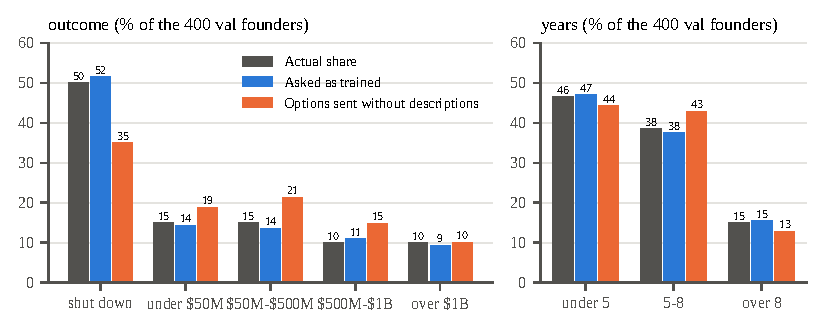
\includegraphics[width=\textwidth]{figures/band_shares.pdf}
\caption{The production model on validation: mean predicted share of each band, asked as trained
(with option descriptions) and with the descriptions removed, against the actual share.}
\label{fig:bands}
\end{figure}

\section{Discussion}

\paragraph{Calibration without discrimination.} Fine-tuning a small decision model on 2,000
founders made it the best-calibrated learn stage but did not make it rank better than a linear
combiner. On this dataset the reason is visible: the signal in the answers is largely additive
and close to the attainable ceiling, so there was little for a more flexible learner to find. The
practical value of a calibrated learn stage is downstream: a policy can pick thresholds for a
target precision, and an agent's ``advance'' and ``pass'' actions inherit honest odds.

\paragraph{Timidity is a policy problem.} A calibrated model whose scores stay near the base rate
supports few confident decisions. Fixed thresholds tuned on small validation sets then become
fragile, as \cond{C3}'s drop from 0.59 to 0.33 precision shows. Applications should expose the
whole precision--recall trade-off (we ship a table of precision and recall at every threshold, per
target and timeline, from validation) rather than a single cut-off.

\paragraph{When do the questions help?} Kev reading the profile did as well as Kev reading TRL's
answers. The questions' role here is explanation: named factors that an investor can inspect and
flip in what-if analyses. Longer, messier real profiles, where an LLM's questions compress
evidence a 0.6B model cannot read directly, may change this.

\paragraph{Request format is part of the model.} A decision model's request carries more than the
state: the question wording and the option descriptions are inputs the model was trained on.
Pipelines that build requests from a reduced representation (labels only) silently change the
input distribution. Checking a served model end to end against offline predictions caught this
before deployment.

\section{Limitations}

\begin{itemize}
\item \textbf{Mostly synthetic data.} 2,950 of 3,000 outcomes come from a known rule plus noise; the
  results describe this dataset, not real founders. No real-world accuracy is claimed. VCBench is
  the intended real test.
\item \textbf{An open 0.6B answerer.} Kev-0.6B, not Jev, answers TRL's questions, so the baselines
  are TRL with a small open answerer rather than TRL as Vela Research runs it.
\item \textbf{Small positive class.} 120 test and 80 validation successes give wide intervals; many
  differences we cannot detect may still exist.
\item \textbf{Limited compute.} Free T4 GPUs in fp32, at most two epochs per fine-tune, one model
  size, one seed. Longer training, larger Kev models, or other calibration methods were not tried.
\item \textbf{The 40-question cap} is a deviation from TRL's defaults, made for compute; \cond{C1a-40}
  measures its cost.
\item \textbf{Production model numbers are validation-only.} The same 400 founders chose its
  checkpoint, fitted its temperatures and measured it.
\end{itemize}

\section{Conclusion}

As TRL's learn stage, a fine-tuned 0.6B decision model is a drop-in, well-calibrated alternative
to the elastic net, but on this data it is not more accurate, and its probabilities are compressed
towards the base rate. Every learn stage is already close to the ceiling the data allows. For
autonomous screening agents this argues for calibrated learn stages with policies built on the full
precision--recall curve, for checking served models end to end, and for testing on real outcomes
(VCBench) where non-additive signal may give flexible learn stages more to find.

\section*{Reproducibility and availability}

Code, data, cached answer matrices, every prediction and every result:
\url{https://github.com/Sidi3355/trl-for-angels} (research branch
\texttt{claude/determined-albattani-dl2cyy}; decision log \texttt{results/DECISIONS.md}; GPU run
logs on branch \texttt{kaggle-results}). TRL fork with the decision combiner and choice-option
descriptions: \url{https://github.com/Sidi3355/think-reason-learn}, branch
\texttt{feature/decision-combiner}. Fine-tuned models:
\href{https://huggingface.co/Sidi3355/trl-for-angels-kev-c3}{\texttt{Sidi3355/trl-for-angels-kev-c3}},
\href{https://huggingface.co/Sidi3355/trl-for-angels-kev-c4}{\texttt{-c4}} and
\href{https://huggingface.co/Sidi3355/trl-for-angels-kev-prod}{\texttt{-prod}}. All seeds are 42.
Compute: about 9 hours of free Kaggle T4 time and 33 minutes of CPU; API cost about \$0.60.

\section*{Acknowledgements}

We thank Vela Research for TRL and Jared Palmer for Kev.

\bibliography{refs}
\bibliographystyle{iclr2026_conference}

\clearpage
\appendix

\section{Validation results}

\begin{table}[h]
\centering\small
\caption{Validation results (400 founders, 80 successes), F0.5-best threshold on validation itself.
These numbers chose the production model's input; test was read afterwards.}
\label{tab:val}
\begin{tabular}{@{}l c c c c c c@{}}
\toprule
Condition & F0.5 & Precision & Recall & Brier & ECE & PR-AUC \\
\midrule
\cond{C1a} & 0.446 & 0.556 & 0.250 & 0.143 & 0.030 & 0.403 \\
\cond{C1a-40} & 0.426 & 0.432 & 0.400 & 0.145 & 0.036 & 0.394 \\
\cond{C1b} & 0.377 & 0.358 & 0.475 & 0.215 & 0.220 & 0.321 \\
\cond{CTRL} & 0.457 & 0.594 & 0.237 & 0.141 & 0.035 & 0.423 \\
\cond{C2} & 0.340 & 0.304 & 0.650 & 0.214 & 0.247 & 0.330 \\
\cond{EXTRA} & 0.400 & 0.400 & 0.400 & 0.383 & 0.454 & 0.323 \\
\cond{C3} & 0.426 & 0.593 & 0.200 & 0.146 & 0.024 & 0.403 \\
\cond{C4} & 0.428 & 0.472 & 0.312 & 0.146 & 0.025 & 0.404 \\
\bottomrule
\end{tabular}
\end{table}

\section{Fine-tuning details}

\begin{table}[h]
\centering\small
\caption{Kev fine-tuning on a Kaggle T4 (fp32). Validation log-loss of the released checkpoint and
after each epoch (lower is better; a constant 20\% guess scores 0.500 on the yes/no task), the
chosen checkpoint, its temperature, and validation ECE before and after temperature scaling.}
\resizebox{\textwidth}{!}{%
\begin{tabular}{@{}l c c c c c c c@{}}
\toprule
Model & Released & Epoch 1 & Epoch 2 & Chosen & Temperature & ECE raw $\to$ cal. & Min/epoch \\
\midrule
\cond{C3} (answers, 873 tokens) & 0.618 & 0.458 & 0.455 & ep2 & 1.072 & 0.031 $\to$ 0.024 & 49 \\
\cond{C4} (profile, $\sim$170 tokens) & 1.086 & 0.475 & 0.470 & ep2 & 1.275 & 0.058 $\to$ 0.025 & 8.5 \\
Production (two questions) & 2.010 & 1.172 & 1.163 & ep2 & 1.149 / 0.871 & 0.027 $\to$ 0.021 & 87 \\
\bottomrule
\end{tabular}}
\end{table}

\section{The best questions}

\begin{table}[h]
\centering\small
\caption{The five questions with the best F0.5 on train (Kev's first five), treating a \emph{yes}
as a prediction of success, with the elastic net's weights on all questions (\cond{C1a}) and on the
40 (\cond{C1a-40}); a blank weight is zero. Near-duplicates (ranks 3--5) share weight.}
\begin{tabularx}{\textwidth}{@{}r X c c c c c@{}}
\toprule
\# & Question & Prec. & Rec. & F0.5 & \cond{C1a} & \cond{C1a-40} \\
\midrule
1 & Is the startup's industry in enterprise/B2B infrastructure (e.g., cybersecurity, cloud infrastructure, logistics, banking technology, energy storage, drug discovery)? & 0.29 & 0.43 & 0.31 & +0.66 & +0.97 \\
2 & Did the founder spend 5+ years at a single employer in the same industry as the current startup? & 0.27 & 0.55 & 0.30 & +1.18 & +1.50 \\
3 & Does the text list at least one prior startup founded by the founder that was acquired? & 0.29 & 0.32 & 0.29 & & +0.03 \\
4 & Does the profile list a prior startup that the founder founded which was acquired or went public? & 0.29 & 0.32 & 0.29 & & $-$0.17 \\
5 & Does the profile list a prior startup founded by the founder that was acquired? & 0.29 & 0.32 & 0.29 & $-$0.19 & $-$0.13 \\
\bottomrule
\end{tabularx}
\end{table}

\section{Compute and cost}

\begin{center}\small
\begin{tabular}{@{}l l@{}}
\toprule
Step & Resource \\
\midrule
Question writing, 2,000 founders (Claude Opus 5.5) & \$0.49 \\
TRL smoke test, 20 founders & \$0.11 \\
RRF fits and answer matrices (all splits) & 86 min, Kaggle T4 \\
Fine-tuning \cond{C3} and \cond{C4}, scoring & 2 h 13 min, two Kaggle T4s \\
Production model & 3 h 16 min, Kaggle T4; 33 min CPU rescoring \\
\bottomrule
\end{tabular}
\end{center}

\end{document}
